\chapter{非稳态热传导}
\thispagestyle{empty}

\section{非稳态导热的基本概念}
\subsection{非稳态导热过程的类型及特点
}

\begin{enumerate}[1. ]
	\item \textbf{非稳态导热过程的类型}
	\begin{itemize}
		\item 温度随时间逐渐趋于恒定(课程要求)
		\item 温度随时间呈现周期性变化
	\end{itemize}
	
	\item \textbf{非稳态导热过程的特点}
	\begin{itemize}
		\item 非稳态导热过程中热量传递方向上不同位置的导热量是处处不同的
		\item 不同位置导热量的差别用于(或来自)该两位置间物体热力学能的变化
	
	\end{itemize}

	\item \textbf{举例}\\
	\hspace*{2em} 复合平壁,初始温度为$t_0$,左侧表面突然升高到$t_1$并保持不变,右侧表面仍与温度为$t_0$的空气接触。
	
	\item \textbf{对于第一种类型的非稳态导热过程,温度分布可以分为两个阶段}
	\begin{itemize}
		\item \textcolor{red}{非正规状况阶段} \quad 
该阶段温度分布主要受初始温度分布的控制
		\item \textcolor{red}{正规状况阶段} \quad  该阶段温度分布主要受热边界条件的影响
	\end{itemize}
\end{enumerate}

\subsection{导热微分方程解的唯一性定律}
假设物体的热物性为常数,则非稳态导热微分方程为
\begin{equation}
	\dfrac{\partial t}{\partial \tau} = a \nabla^2 t + \dfrac{\dot{\varPhi}}{\rho c}
\end{equation}
数学上可以证明,若某一函数$t(x,y,z,\tau)$满足上述方程以及一定的初始条件和边界条件,则此函数就是这一特定导热问题的唯一解。即\textcolor{red}{不可能同时存在两个都满足导热微分方程及同一定解条件的不同的解。}

这个结论称为\dy[解的唯一性定律]{JDWYXDL}。本章所讨论的各种分析解都被认为是满足特定问题的唯一解。
\vspace*{0.5em}

\subsection{第三类边界条件下的非稳态导热}
第三类边界条件为
\begin{equation}
	- \lambda \left(\dfrac{\partial t}{\partial n}\right)_\w = h(t_\w - h_\f)
\end{equation}

初始温度为$t_0$、导热系数为$\lambda$、厚度为$2\delta$的平板,突然将它置于温度为$t_\infty$的流体中进行冷却,表面传热系数为$h$,根据\textcolor{red}{平板内部导热热阻与表面对流传热热阻的比值(即$Bi$毕渥数)}的不同,平板中温度场变化过程会出现三种情形,如图\ref{Bi}.

\begin{enumerate}[1.]
	\item $\bm{\dfrac{\delta}{\lambda} >> \dfrac{1}{h} \quad(Bi \to \infty)}$\\[0.5em]
	\hspace*{2em}表面对流传热热阻几乎可以忽略,因而过程一开始平板的表面温度就被冷却到$t_\infty$。随着时间的推移,平板内部各点的温度逐渐下降而趋近于$t_\infty$。
	\vspace*{1em}
	
	\item $\bm{\dfrac{\delta}{\lambda} << \dfrac{1}{h} \quad(Bi \to 0)}$\\[0.5em]
	\hspace*{2em}平板内部导热热阻几乎可以忽略,因而任一时刻平板中各点的温度接近均匀,并随着时间的推移整体下降,逐渐趋近于$t_\infty$。
	\vspace*{1em}
	
	\item $\bm{\dfrac{\delta}{\lambda} \approx \dfrac{1}{h} \quad(Bi \approx 1)}$\\[0.5em]
	\hspace*{2em}平板中温度场变化过程介于上述两种极端情况之间。
	
\end{enumerate}
\begin{figure}[!htb]
	\centering
	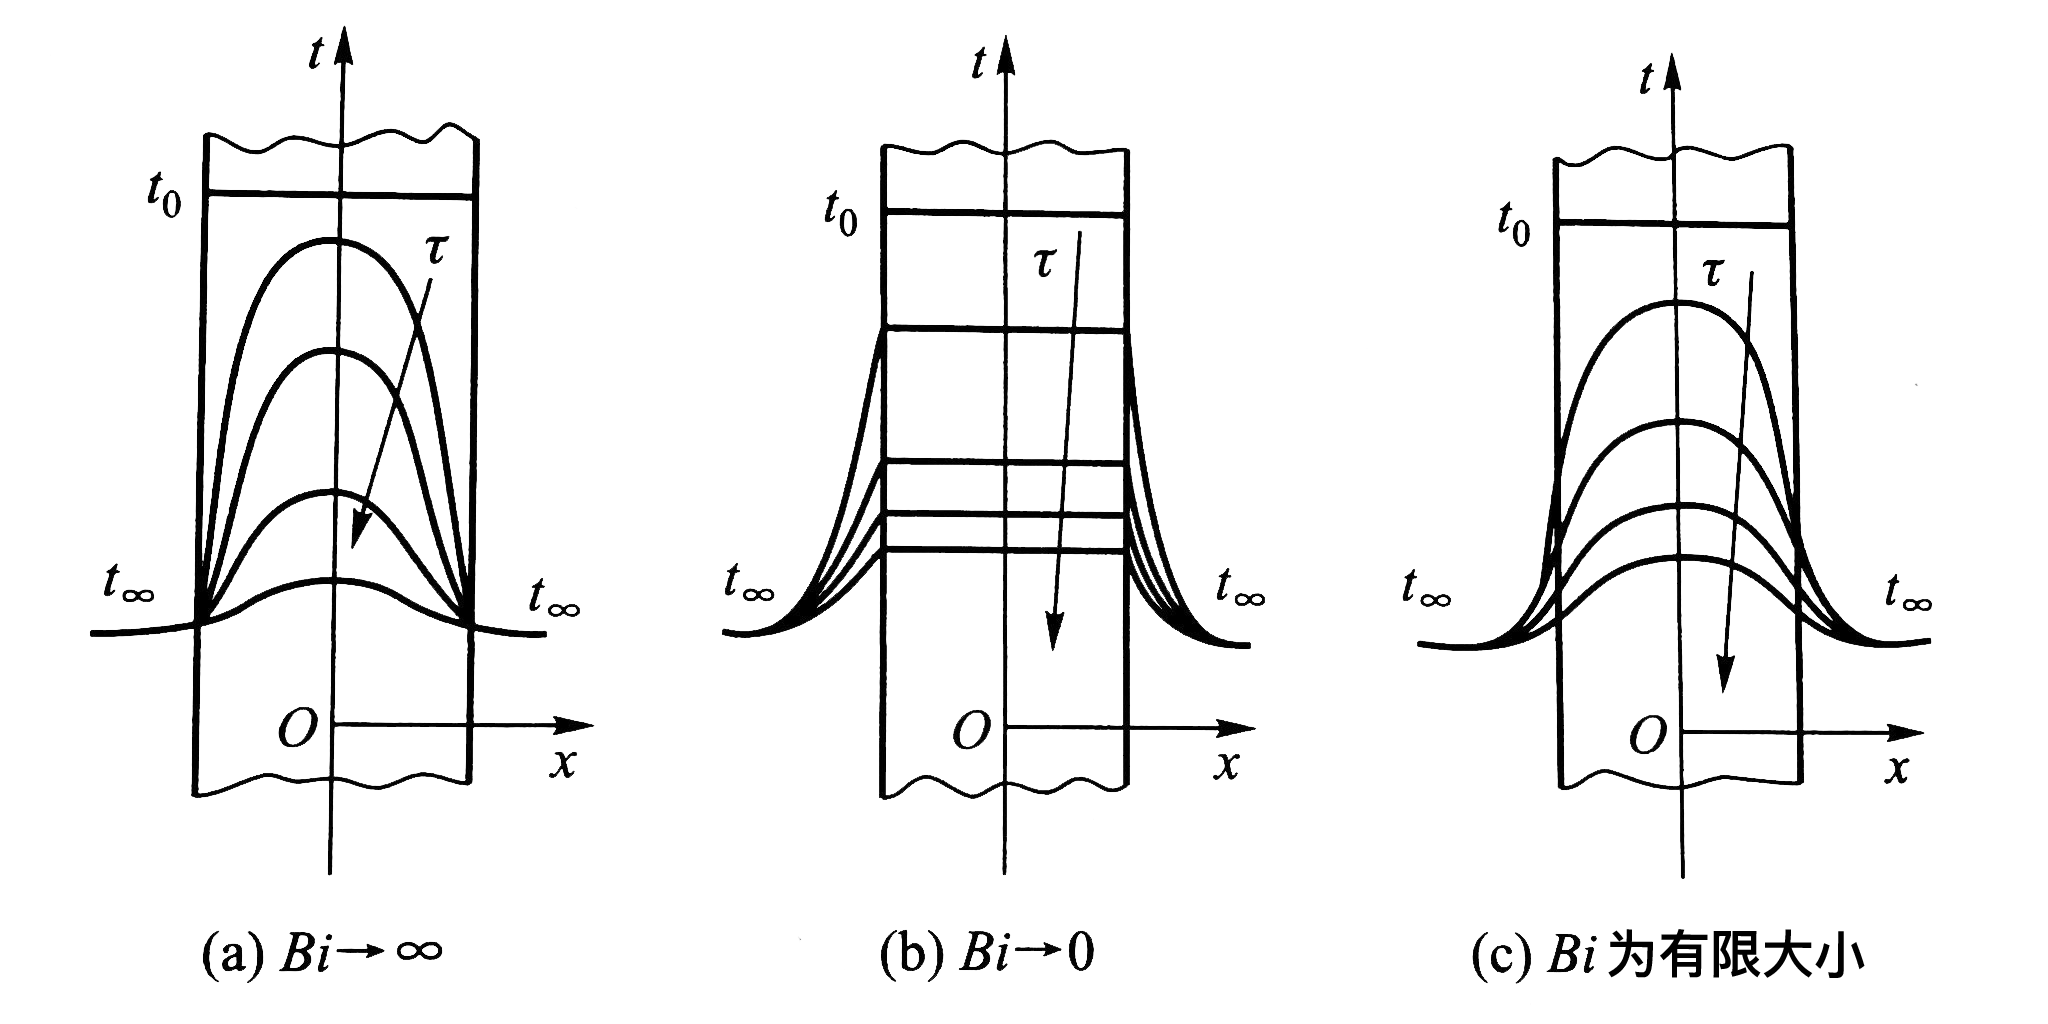
\includegraphics[width=0.7\linewidth]{pic/Bi.png}
	\vspace*{-1em}
	\caption{不同$Bi$数对非稳态导热对影响}
	\label{Bi}
\end{figure}


\section{零维问题的分析法——集中参数法}
\tdefination[零维问题]
当固体内部的导热热阻远小于其表面传热热阻时,任何时刻固体内部的温度都趋于一致,以至于可以认为整个固体在同一瞬时处于同一温度下,此时可视为\dy[零维问题]{LWWT}。

\defination[集中参数法]
针对零维问题忽略物体内部导热热阻的简化分析方法。\index{JZCSF@集中参数法}
\vspace*{0.5em}

\subsection{集中参数法的温度场分析解}
\begin{enumerate}[\textbf{步骤} 1 ]
	\item \textbf{提出问题}\\
	\hspace*{2em} 内部导热热阻可忽略的物体,初始温度为$t_0$,突然将它置于温度恒为$t_\infty$的流体中,设$t_0 > t_\infty$ ,求物体温度随时间的变化。
	
	\item \textbf{导出简化的微分方程}
	\begin{itemize}
		\item 等效内热源法
		\[
			\dfrac{\partial t}{\partial \tau} = a \nabla^2 t + \dfrac{\dot{\varPhi}}{\rho c} \quad\quad a \nabla^2 t = 0 
			\quad\quad - \dot{\varPhi} = hA(t - t_\infty)
		\]
		即
		\begin{equation}
			\rho c V\dfrac{\d t}{\d \tau} = - h A(t - t_\infty)
		\end{equation}
		
		\item 能量守恒法
		\begin{equation}
			\rho c V\dfrac{\d t}{\d \tau} = - h A(t - t_\infty)
		\end{equation}
	\end{itemize}
	
	\item \textbf{列出定解问题}
	\begin{equation}
		\begin{cases}
			\, \rho c V\dfrac{\d t}{\d \tau} = - h A \theta \\
			\theta = t - t_\infty \\
			\theta(0) = t_0 - t_\infty = \theta_0
		\end{cases}
	\end{equation}
	
	\item \textbf{求解方程}\\
	求解方程,解得\textbf{温度场分析解}为
	\begin{equation}
		\dfrac{\theta}{\theta_0} = \exp\left(- \dfrac{hA}{\rho c V} \tau \right)
	\end{equation}
	定义$l_\text{c} = \dfrac{V}{A}$,\dy[毕渥数]{BWS}$Bi = \dfrac{h l_\text{c}}{\lambda}$,\dy[傅立叶数]{FLYS}$Fo = \dfrac{a \tau}{l_{\text{c}}^2}$,则
	\begin{equation}
		\dfrac{\theta}{\theta_0} = \exp\left(- \dfrac{hA}{\rho c V} \tau \right) = \exp\left(- \dfrac{hl_\text{c}}{\lambda} \cdot \dfrac{\lambda}{\rho c} \cdot \dfrac{\tau}{l_{\text{c}}^2} \right) = \exp\left(- \dfrac{hl_\text{c}}{\lambda} \cdot \dfrac{a \tau}{l_{\text{c}}^2} \right) = \exp (-Bi\cdot Fo)
	\end{equation}
	
	\begin{figure}[!htb]
		\centering
		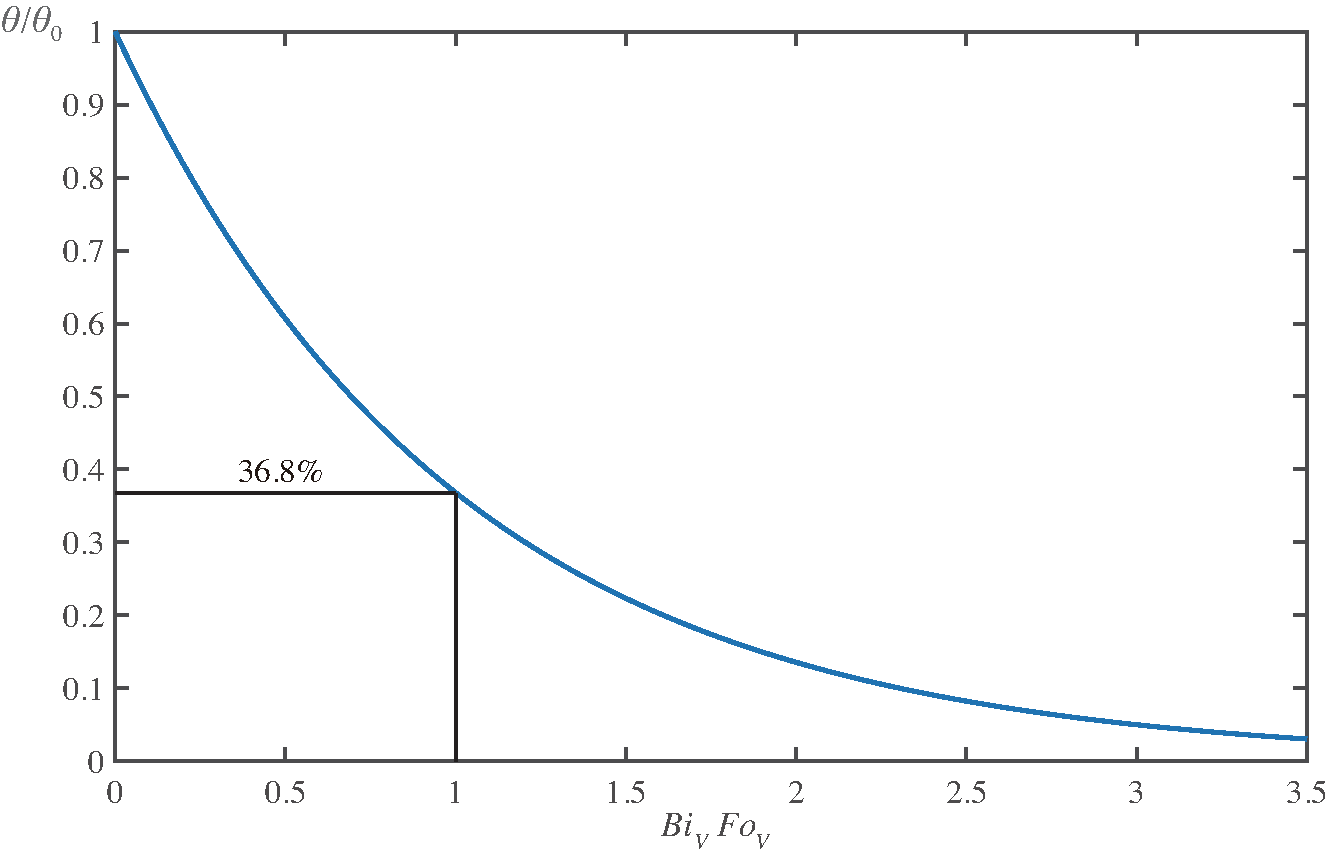
\includegraphics[width=0.7\linewidth]{pic/集中参数法.pdf}
		\vspace*{-1em}
		\caption{集中参数法求解结果图}
		\label{集中参数法}
	\end{figure}
	
	其中,各个物理量的意义为
	\begin{enumerate}[\hspace*{2em}(1) ]
		\item \textbf{时间常数$\bm{\tau_0}$}
		\begin{itemize}
			\item 当$\tau_\text{c} = \dfrac{\rho cV}{hA}$时,有
			\begin{equation}
				\dfrac{\theta}{\theta_0} = \exp(-1) \approx 0.368 = 36.8\%
			\end{equation}
		$\tau_\text{c} = \dfrac{\rho cV}{hA}$称为\dy[时间常数]{SJCS},即过余温度变到初始过余温度
		的36.8\%所需的时间
		\item 时间常数取决于导热固体的热容($\rho cV$)以及表面传热条件($hA$)
		\end{itemize}
	
	\item \textbf{毕渥数$\bm{Bi}$}
	\begin{equation}
		Bi = \dfrac{h l_\text{c}}{\lambda} = \dfrac{l_\text{c}/\lambda}{1/h}
	\end{equation}
	毕渥数的物理意义:导热物体的内部导热热阻与表面对流传热热阻的比值

	\item \textbf{傅立叶数$\bm{Fo}$}
	\begin{equation}
		Fo = \dfrac{a \tau}{l_{\text{c}}^2} = \dfrac{\tau}{l_{\text{c}}^2 / a}
	\end{equation}
	傅立叶数的物理意义:热扰动作用时间与热扰动扩散到$l_{\text{c}}^2$面积上所需时间的比值
	\end{enumerate}

	由温度场分析解,可得\textbf{导热热流量}为
	\begin{equation}
		\varPhi = hA(t - t_\infty) = hA(t_0 - t_\infty) \exp\left(- \dfrac{hA}{\rho c V} \tau \right)
	\end{equation}
	\textbf{导热量}为
	\begin{equation}
		Q_{\tau} = \int_{0}^\tau \varPhi \, \d \tau =  (t_0 - t_\infty) \rho c V\left[1 -\exp\left(- \dfrac{hA}{\rho c V} \tau \right) \right]
	\end{equation}
\end{enumerate}
\warn[
{
\begin{enumerate}[1.]
	\item 集中参数法适用的条件是\textcolor{red}{$Bi$数很小}
	\item 当按特征长度$l$定义的$Bi$数满足
	\begin{equation}
		Bi = \dfrac{hl}{\lambda} \le 0.1
	\end{equation}
	时,采用集中参数法计算的误差满足工程要求
	\item 常见导热体的特征长度
	\begin{equation}
		\begin{cases}
			\, l = \delta, & \mbox{厚度为}2\delta\mbox{的平板}\\
			\, l = R, & \mbox{底面半径为}R\mbox{的圆柱}\\
			\, l = R, & \mbox{半径为}R\mbox{的球}
		\end{cases}
	\end{equation}
\end{enumerate}
}
]

\section{典型一维物体非稳态导热的分析解}
\subsection{三种几何形状物体的温度场分析解}
\noindent \textbf{1. 平板}\\
\hspace*{2em} 初始温度为$t_0$,导热系数为$\lambda$,厚度为$2\delta$的无限大平板;突然将其置于温度为$t_\infty$的流体中,表面传热系数为$h$;假定热物性为常数,无内热源。可以列出定解问题
\begin{equation}
	\begin{cases}
		\, \dfrac{\partial t}{\partial \tau} = a \dfrac{\partial^2 t}{\partial x^2}, &0 < x < \delta , \tau > 0\\[0.5em]
		\, t(x,0) = t_0, & 0 \le x \le \delta\\[0.5em]
		\, \left. \dfrac{\partial t(x, \tau)}{\partial x} \right|_{x = 0} = 0,\\[0.7em]
		\, -\lambda \left. \dfrac{\partial t(x, \tau)}{\partial x} \right|_{x = \delta} = h\left[t(\delta, \tau) - t_\infty \right].
	\end{cases}
\end{equation}
引入过余温度
\begin{equation}
	\theta = t(x, \tau) - t_\infty
\end{equation}
定解问题化为
\begin{equation}
	\begin{cases}
		\, \dfrac{\partial \theta}{\partial \tau} = a \dfrac{\partial^2 \theta}{\partial x^2}, &0 < x < \delta , \tau > 0\\[0.5em]
		\, \theta(x,0) = \theta_0, & 0 \le x \le \delta\\[0.5em]
		\, \left. \dfrac{\partial \theta(x, \tau)}{\partial x} \right|_{x = 0} = 0, & \tau > 0\\[1em]
		\, -\lambda \left. \dfrac{\partial t(x, \tau)}{\partial x} \right|_{x = \delta} = h\theta(\delta, \tau). & \tau > 0
	\end{cases}
\end{equation}
由数学物理方法中的分离变量法,解得
\begin{align}
	\dfrac{\theta(x,\tau)}{\theta_0} &= \sum_{n = 1}^{\infty} C_n \e^{- \mu_n^2 Fo} \cos(\mu_n\eta)\\
	C_n &= \dfrac{2 \sin \mu_n}{\mu_n + \cos \mu_n \sin \mu_n}
\end{align}
$\mu_n$为下列特征方程的根
\begin{align}
	\tan \mu_n = \dfrac{Bi}{\mu_n}, \,\, n = 1,2,\cdots
\end{align}
其中,$Fo = \dfrac{a \tau}{\delta^2},\,\, \eta = \dfrac{x}{\delta}, \,\, Bi = \dfrac{h \delta}{\lambda}$.
\vspace*{1em}

\noindent \textbf{2. 圆柱和球}

同理可得圆柱和球的分析解如表\ref{典型一维非稳态导热}.

\begin{table}[!htb]
	\centering\setlength{\tabcolsep}{4mm}{
		\begin{tabular}{cccccc}
			\toprule
			几何形状 & 无量纲温度分析解 &  $\mu_n$是对应的特征方程 & $\eta$ & $Fo$ & $Bi$\\
			\midrule
			&&&&&\\[-1.5em]
			圆柱 & \makecell[c]{$\displaystyle \dfrac{\eta,\tau}{\theta_0} = \sum_{n = 1}^{\infty} C_n \e^{-\mu_n Fo}J_0(\mu_n\eta)$\\[1.2em]$\displaystyle C_n = \dfrac{2}{\mu_n} \dfrac{J_1(\mu_n)}{J_0^2(\mu_n) + J_1^2(\mu_n)}$} & $\displaystyle \mu_n \dfrac{J_1(\mu_n)}{J_2(\mu_n)} = Bi,\,\, n = 1,2,\cdots$ & $\dfrac{r}{R}$ & $\dfrac{a \tau}{R^2}$ & $\dfrac{hR}{\lambda}$ \\[3em]
			\hline
			&&&&&\\[-1.25em]
			球 & \makecell[c]{$\displaystyle \dfrac{\eta,\tau}{\theta_0} = \sum_{n = 1}^{\infty} C_n \e^{-\mu_n Fo}\dfrac{1}{\mu_n \eta} \sin(\mu_n\eta) $\\[1.2em]$\displaystyle C_n =2 \dfrac{\sin\mu_n - \mu_n \cos (\mu_n)}{\mu_n - \sin \mu_n \cos \mu_n}$} & $\displaystyle 1 -  \mu_n \cos \mu_n = Bi,\,\, n = 1,2,\cdots$ & $\dfrac{r}{R}$ & $\dfrac{a \tau}{R^2}$ & $\dfrac{hR}{\lambda}$ \\[2.75em]
			\bottomrule
		\end{tabular}
		\caption{圆柱和球在第3类边界条件下非稳态导热无量纲温度的分析解}
		\label{典型一维非稳态导热}
	}
\end{table}

\subsection{非稳态导热正规状况阶段分析解的简化}
当初始条件对无量纲温度分布影响基本消失时,称为\dy[非稳态导热正规状况阶段]{FWTDRZGZKJD}。

对于非周期性的非稳态导热过程,从过程开始到温度分布趋近于稳态分布的时间间隔中,初始条件影响基本消失的阶段占了极大部分的比例,故称这一阶段为\textcolor{red}{“正规状况”}
。

对于平板,$Bi=1.0$时,$\tan \mu_n = \dfrac{Bi}{\mu_n}, n =1,2,\cdots$的前4个根分别为为0.8603, 3.4256, 6.4373, 9.5293,可见$\mu_n$的值随$n$的增加而迅速增加。这导致分析解$\dfrac{\Theta(x,\tau)}{\Theta_0}=\displaystyle \sum_{n=1}^{\infty} C_n\exp\big(-\mu_n^2Fo\big) \cos (\mu_n \eta)$的无穷级数第一项以后的各项在$Fo$数较大时迅速衰减。


数值计算表明,当$Fo$大于0.2以后,略去无穷级数中第二项及以后各项所得的计算结果与按完整级数所得的计算结果的偏差小于$1\%$。这相当于将无穷级数解中的系数$C_n(n \ge 2)$取为零。而   的无穷系列值是为了使分析解满足初始条件而引入的,这样的处理意味着基本略去初始条件的影响(而不会带来较大偏差),所以\textbf{分析解无穷级数的第一项就是正规状况阶段的解}。

所以,各个形状的非稳态导热正规状况阶段分析解可以统一表示为
\begin{align}
	\dfrac{\Theta(\eta, \tau)}{\Theta_0} &= A\exp\big(-\mu_1^2 Fo\big) f(\mu_1 \eta)\\[0.5em]
	\dfrac{Q}{Q_0} &= 1 - A\exp\big(-\mu_1^2Fo\big)B
\end{align}
其中,各个参数如表\ref{正规状况非稳态导热}.
\begin{table}[!htb]
	\centering\setlength{\tabcolsep}{8mm}{
		\begin{tabular}{cccc}
			\toprule
			几何形状 & $A$ & $B$ & $f(\mu_1\eta)$\\
			\midrule
			&&&\\[-1.25em]
			平板 & $2 \dfrac{\sin \mu_1}{\mu_1 + \sin \mu_1 \cos \mu_1}$ & $\dfrac{\sin \mu_1}{\mu_1}$ & $\cos(\mu_1 \eta)$\\
			&&&\\[-0.5em]
			圆柱 & $\dfrac{J_1(\mu_1)}{\mu_1\big[J_0^2(\mu_1)+J_1^2(\mu_1)\big]}$ & $2 \dfrac{J_1(\mu_1)}{\mu_1}$ & $J_0(\mu_1\eta)$ \\
			&&&\\[-0.5em]
			球 & $2\dfrac{\sin \mu_1 - \mu_1 \cos \mu_1}{\mu_1 - \sin \mu_1 \cos \mu_1}$ & $3 \dfrac{\sin \mu_1 - \mu_1 \cos \mu_1}{\mu_1^3}$ & $\dfrac{\sin (\mu_1 \eta)}{\mu_1 \eta}$\\[1em]
			\bottomrule
		\end{tabular}
		\caption{三种形状的非稳态导热正规状况阶段分析解}
		\label{正规状况非稳态导热}
	}
\end{table}

\subsection{非稳态导热正规状况阶段的工程计算方法}

\section{半无限大物体的非稳态导热}
\subsection{半无限大物体的温度场分析解}
有一半无限大物体,初始温度为$t_0$,导热系数为$\lambda$。在$\tau = 0$时刻,$x = 0$的侧面突然受到热扰动。则列出定解问题如下
\begin{itemize}
	\item 导热微分方程
	\begin{equation}
		\dfrac{\partial t}{\partial \tau} = a \dfrac{\partial^2 t}{\partial x^2}\quad (0<x<\infty,\tau > 0)
	\end{equation}
	
	\item 初始条件
	\begin{equation}
		\tau = 0,\,\, t(x, \tau) = t_0
	\end{equation}

	\item 边界条件:下列三个边界条件取一种
	\begin{itemize}
		\item 第一类边界条件
		\begin{equation}
			x = 0, \,\, t(x, \tau) = t_\w
		\end{equation}
		\item 第二类边界条件
		\begin{equation}
			x = 0, \, \, - \lambda \dfrac{\partial t(x, \tau)}{\partial x} = q_0
		\end{equation}
		\item 第三类边界条件
		\begin{equation}
			x = 0, \, \, - \lambda \dfrac{\partial t(x, \tau)}{\partial x} = h \big[t_\infty - t(x, \tau)\big]
		\end{equation}
	\end{itemize}
	
\end{itemize}

\noindent 由数学物理方法,得到三种边界条件下的解为
\begin{itemize}
	\item 第一类边界条件的解
	\begin{equation}
		\dfrac{t(x, \tau)-t_\w}{t_0 - t_\w} = \erf \left(\dfrac{x}{2\sqrt{a\tau}}\right)
	\end{equation}
	\item 第二类边界条件的解
	\begin{equation}
		t(x, \tau)  - t_0 = \dfrac{2 q_0 \sqrt{\dfrac{a \tau}{\pi}}}{\lambda} \exp \left(-\dfrac{x^2}{4 a \tau}\right) - \dfrac{q_0 x}{\lambda} \erfc \left(\dfrac{x}{2\sqrt{a \tau}}\right)
	\end{equation}
	\item 第三类边界条件的解
	\begin{equation}
		\dfrac{t(x, \tau) - t_0}{t_\infty - t_0} = \erfc\left(\dfrac{x}{2\sqrt{a \tau}}\right) - \exp\left(\dfrac{hx}{\lambda} + \dfrac{h^2 a \tau}{\lambda^2}\right)\erfc \left(\dfrac{x}{2\sqrt{a\tau}} + \dfrac{h\sqrt{a \tau}}{\lambda}\right)
	\end{equation}
\end{itemize}

其中$\erf\left(\dfrac{x}{2\sqrt{a \tau}}\right)$称为\dy[误差函数]{WCHS},$\erfc\left(\dfrac{x}{2 \sqrt{a \tau}}\right) = 1 - \erf\left(\dfrac{x}{2\sqrt{a \tau}}\right)$称为\dy[余误差函数]{YWCHS}。
\vspace{1em}

\subsection{半无限大物体的导热量计算式}
\noindent 以第一类边界条件的解为例,计算半无限大物体的导热量:
\begin{enumerate}[\hspace*{2em} (1) ]
	\item 通过$x$截面的导热热流密度为
	\begin{equation}
		q_x = \lambda \dfrac{t_\w - t_0}{\sqrt{\pi a \tau}} \exp \left( - \dfrac{x^2}{4 a \tau}\right)
	\end{equation}

	\item 表面的导热热流量为
	\begin{equation}
		\varPhi_\m = Aq_\m = A \lambda \dfrac{t_\w - t_0}{\sqrt{\pi a \tau}}
	\end{equation}

	\item 表面的导热热量(导热量)为
	\begin{equation}
		Q_\w = \int_0^\tau \varPhi_\m \, \d \tau = 2A\sqrt{\dfrac{\tau}{\pi}}\sqrt{\rho c \lambda}(t_\w - t_0)
	\end{equation}
	
\end{enumerate}



\subsection{分析解的讨论}
以第一类边界条件的解为例,讨论无量纲常数$\eta = \dfrac{x}{2\sqrt{a \tau}}$的物理意义:
\begin{equation}
	\dfrac{t(x, \tau)-t_\w}{t_0 - t_\w} = \erf \left(\dfrac{x}{2\sqrt{a\tau}}\right) \quad \Rightarrow \quad 
	\left(\dfrac{x}{2\sqrt{a \tau}}\right)= 2, \,\, \dfrac{t(x, \tau)-t_\w}{t_0 - t_\w} = 0.9953
\end{equation}
可以得到
\begin{enumerate}[\hspace*{2em} (1) ]
	\item 从空间上看“半无限大物体”这一模型的适用条件为
	\begin{equation}
		\dfrac{x}{2 \sqrt{a \tau}} \ge 2 \quad \Rightarrow \quad x \ge 4\sqrt{a \tau}
	\end{equation}

	\item 从时间上看“半无限大物体”这一模型的适用条件为
	\begin{equation}
		\dfrac{x}{2 \sqrt{a \tau}} \ge 2 \quad \Rightarrow \quad \tau \ge \dfrac{x^2}{16a}
	\end{equation}
\end{enumerate}


\section{简单几何形状物体多维非稳态导热的分析解}
\noindent 分析方法
\begin{enumerate}[\hspace*{2em} \textbf{方法} 1 ]
	\item \textbf{分析法}\\
	通过数学分析方法求解定解条件下的导热微分方程来获得温度场函数。
	
	\item \textbf{数值法}\\
	通过计算机获得某个计算条件下物体中代表性空间点上的温度值。
\end{enumerate}
\vspace*{0.5em}

\subsection{乘积解法}
多维非稳态导热问题中,几种简单几何形状的物体的非稳态导热问题的分析解可以用几个相应的一维非稳态导热分析解相乘得出,称为\dy[乘积解法]{CJJF}。如图\ref{乘积解法的典型应用},典型应用有

\begin{enumerate}[\hspace*{2em} (1) ]
	\item 前提假设\\
			三个物体初始温度为$t_0$、导热系数为$\lambda$。与周围问题为$t_\infty$的流体发生对流传热,表面传热系数为$h$。物体的热物性为常数,无内热源。
	\item \textbf{无限长方柱}
			\\由两块无限长平板相贯而成。其分析解为
			\begin{equation}
				\varTheta = \dfrac{\theta(x,y,z}{\theta_0} = \varTheta_{\text{p}1}(x, \tau) \cdot \varTheta_{\text{p}2}(y, \tau)
			\end{equation}
	
	\item \textbf{短圆柱}\\
	由一块无限长平板和一个无限长圆柱相贯而成。其分析解为
	\begin{equation}
		\varTheta = \dfrac{\theta(x,y,z}{\theta_0} = \varTheta_{\text{p}}(x, \tau) \cdot \varTheta_{\text{c}}(r, \tau)
	\end{equation}
	
	\item \textbf{短方柱}\\
	由三块无限长平板相贯而成。其分析解为
	\begin{equation}
		\varTheta = \dfrac{\theta(x,y,z}{\theta_0} = \varTheta_{\text{p}1}(x, \tau) \cdot \varTheta_{\text{p}2}(y, \tau)\cdot \varTheta_{\text{p}3}(z, \tau)
	\end{equation}
\end{enumerate}

其中,$ \varTheta_{\text{p}}, \varTheta_{\text{c}}$分别表示一维无限大平板及圆柱在第三类边界条件下无量纲温度的分析解。

\begin{figure}[!htb]
	\centering
	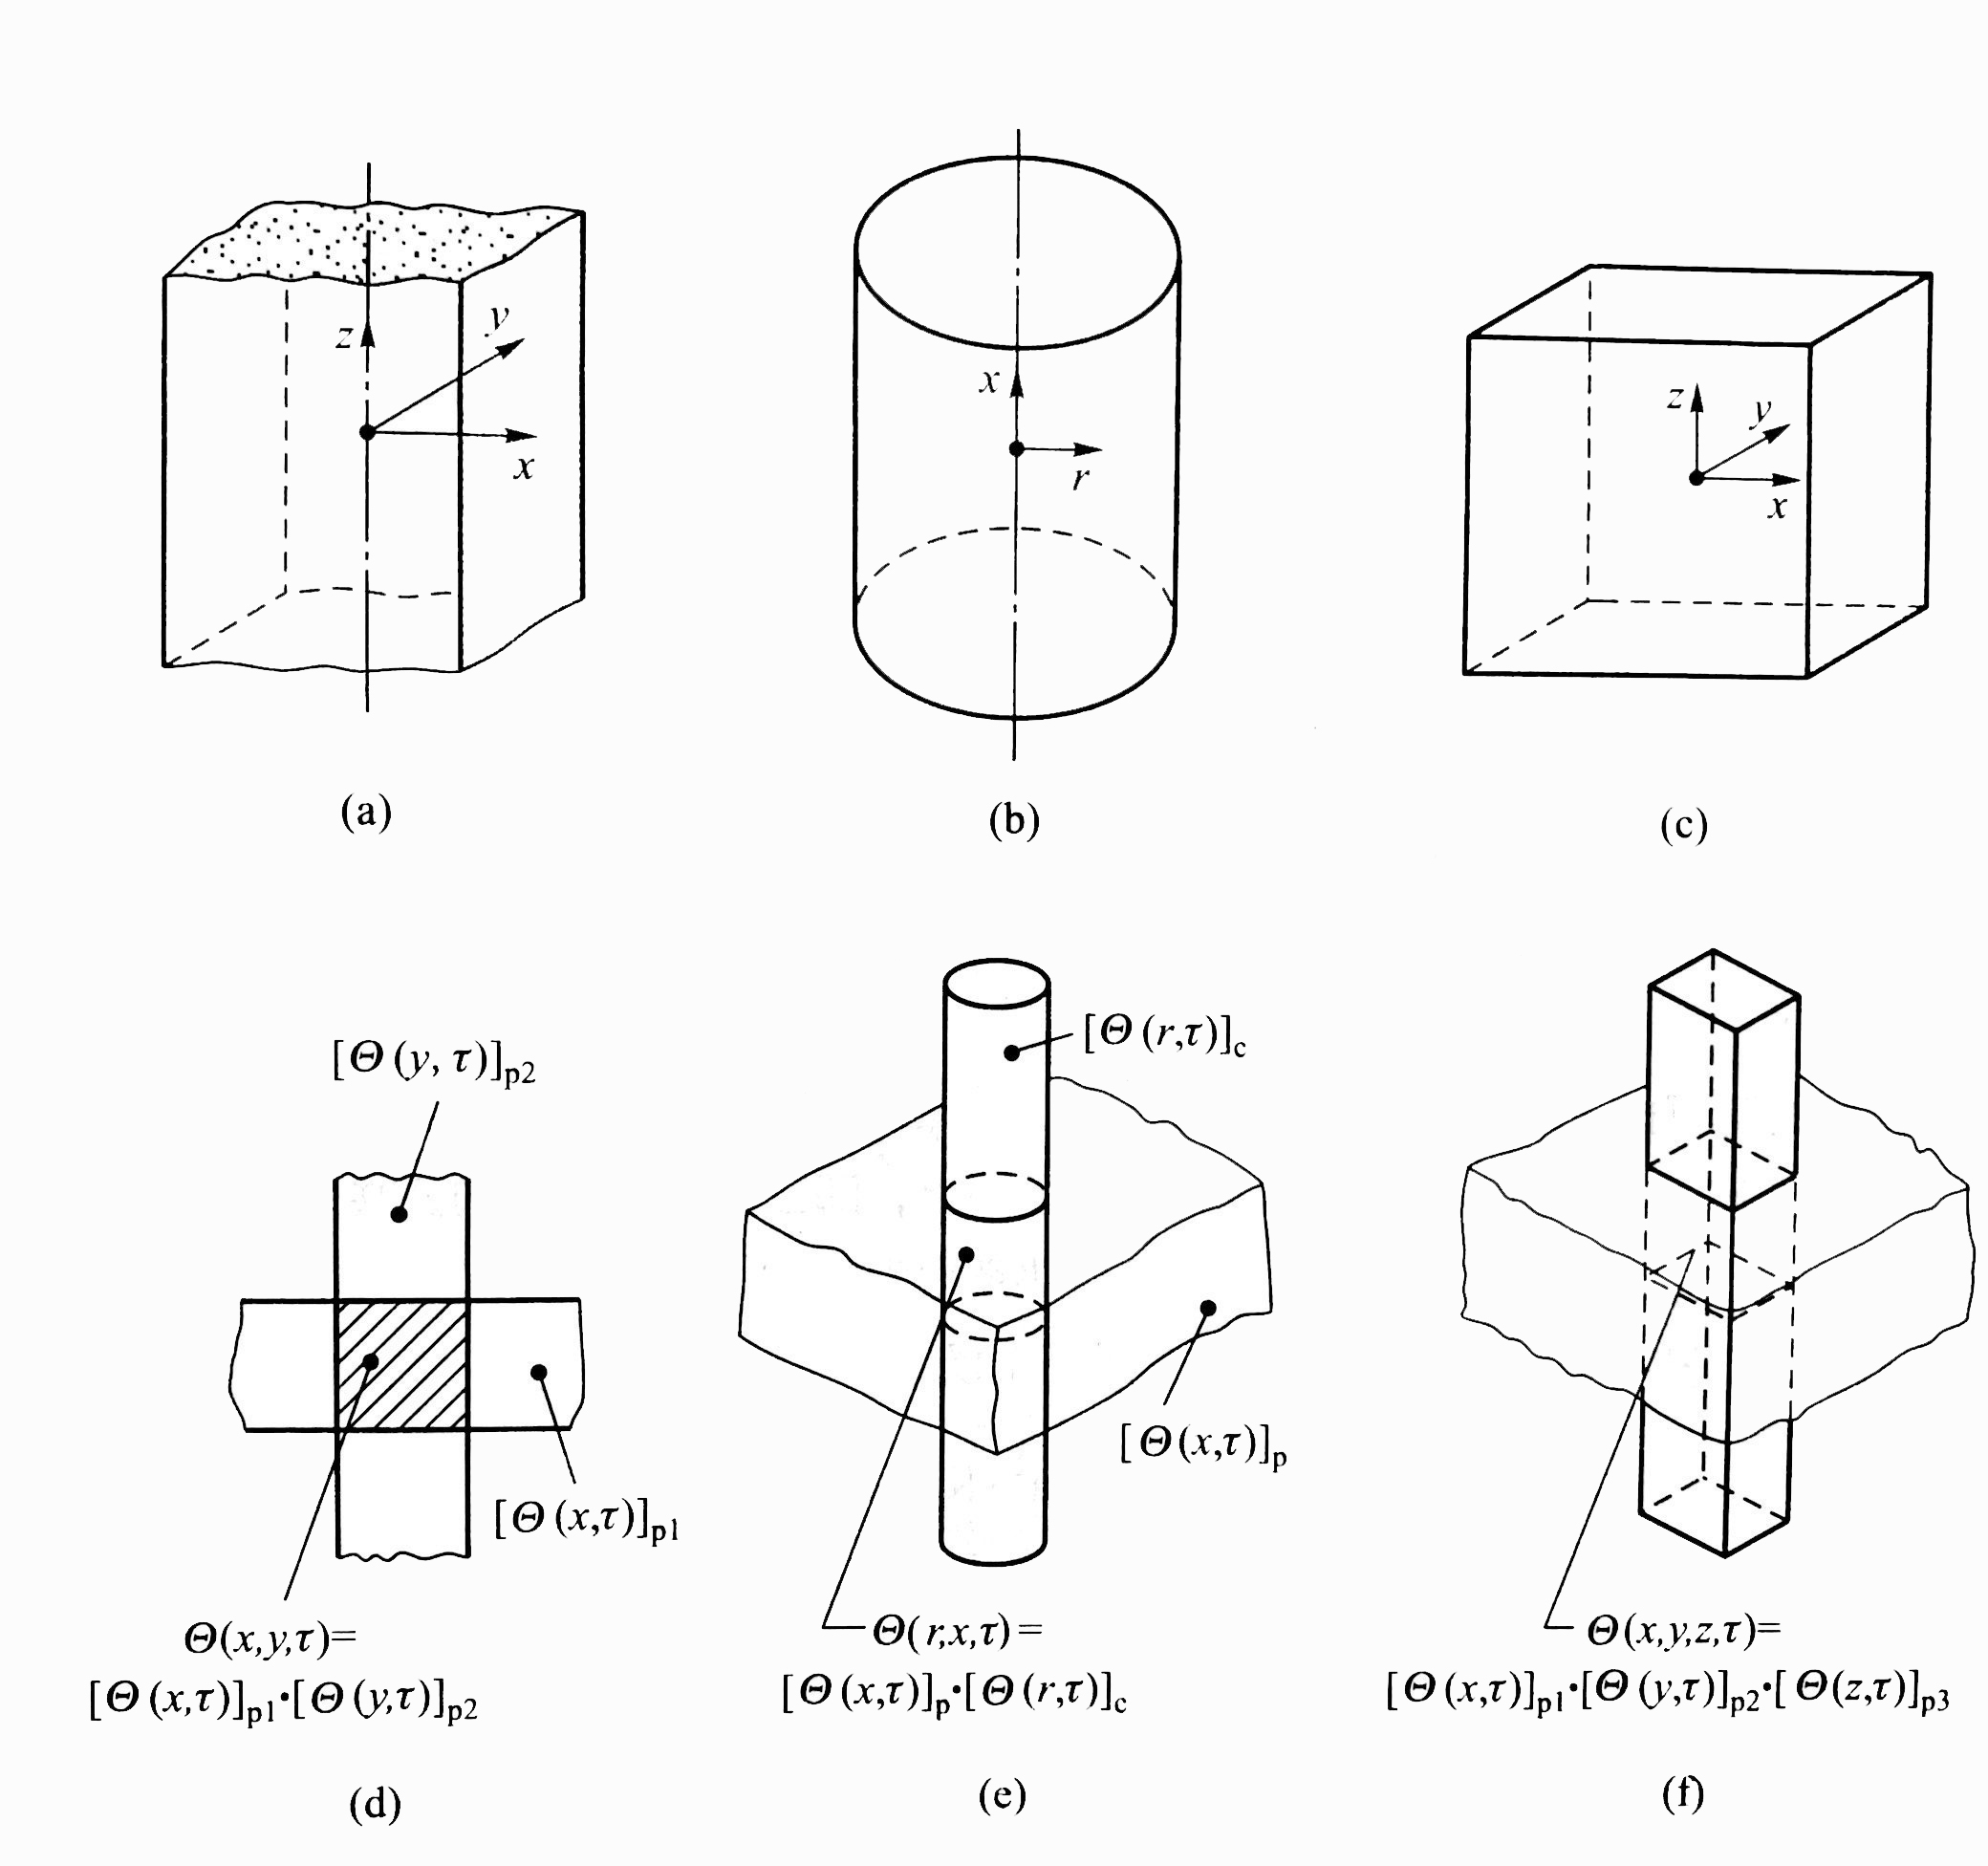
\includegraphics[width=0.7\linewidth]{pic/多维非稳态.jpeg}
	\vspace*{-2em}
	\caption{乘积解法的典型应用}
	\label{乘积解法的典型应用}
\end{figure}

\warn[
\textbf{乘积解法的适用条件}\vspace*{-0.5em}
{
\begin{enumerate}[\hspace*{2em}(1) ]
	\item 只适用于第三类边界条件。特别地,对于$h \to \infty$,即第一类边界条件也适用\vspace*{-0.5em}
	\item 物体初始温度均匀\vspace*{-0.5em}
	\item 周围介质温度均匀\vspace*{-0.5em}
	\item 表面传热系数均匀\vspace*{-0.5em}
	\item 常物性、没有内热源
\end{enumerate}	
}
]
\vspace*{0.5em}

\subsection{多维非稳态导热量的计算}
\begin{enumerate}[\textbf{步骤} 1 ]
	\item \textbf{计算该热量占非稳态导热过程总导热量的百分数}\\
	可以由类似乘积解法的模式导出
	\begin{itemize}
		\item 二维问题
		\begin{equation}
			\dfrac{Q}{Q_0} = \left(\dfrac{Q}{Q_0}\right)_1 + \left(\dfrac{Q}{Q_0}\right)_2 - \left(\dfrac{Q}{Q_0}\right)_1\left(\dfrac{Q}{Q_0}\right)_2 
		\end{equation}
		
		\item 三维问题
		\begin{equation}
		\dfrac{Q}{Q_0} = \left(\dfrac{Q}{Q_0}\right)_1 + \left(\dfrac{Q}{Q_0}\right)_2 + \left(\dfrac{Q}{Q_0}\right)_3 -\left(\dfrac{Q}{Q_0}\right)_1\left(\dfrac{Q}{Q_0}\right)_2 - \left(\dfrac{Q}{Q_0}\right)_1\left(\dfrac{Q}{Q_0}\right)_3 - \left(\dfrac{Q}{Q_0}\right)_2\left(\dfrac{Q}{Q_0}\right)_3
		\end{equation}
	\end{itemize}
	其中,$\left(\dfrac{Q}{Q_0}\right)_1,\left(\dfrac{Q}{Q_0}\right)_2,\left(\dfrac{Q}{Q_0}\right)_3$分别表示构成二维与三维非稳态导热物体的第$1,2,3$个一维几何体的导热量百分数
	
	\item \textbf{从热平衡角度得出总导热量}
	
	\item \textbf{将上述两项相乘得到导热量}
\end{enumerate}






